% Dit werk is gelicenseerd onder de licentie Creative Commons Naamsvermelding-GelijkDelen 4.0 Internationaal. Ga naar http://creativecommons.org/licenses/by-sa/4.0/ om een kopie van de licentie te kunnen lezen.
\documentclass[t]{beamer}

% vaak gebruikte packages, nederlands


\usepackage{a4wide}                     % Iets meer tekst op een bladzijde
\usepackage[dutch]{babel}               % Voor nederlandstalige hyphenatie (woordsplitsing)
%\usepackage{amsmath,amsthm}             % Uitgebreide wiskundige mogelijkheden
%\usepackage{amssymb}                    % Voor speciale symbolen zoals de verzameling Z, R...
%\usepackage{makeidx}                    % Om een index te maken
\usepackage{url}                        % Om url's te verwerken
\usepackage{graphicx,subfigure}         % Om figuren te kunnen verwerken
\usepackage{color}
\usepackage{multicol}
\usepackage[small,bf,hang]{caption}     % Om de captions wat te verbeteren
%\usepackage{xspace}                     % Magische spaties na een commando
\usepackage[latin1]{inputenc}           % Om niet ascii karakters rechtstreeks te kunnen typen
\usepackage{float}                      % Om nieuwe float environments aan te maken. Ook optie H!
\usepackage{flafter}                    % Opdat floats niet zouden voorsteken
\usepackage[section]{placeins}			% Om ervoor te zorgen dat floats binnen dezelfde section blijven
%\usepackage{listings}                   % Voor het weergeven van letterlijke text en codelistings
%\usepackage[numbers]{natbib}            % Voor juiste citatie stijl
\usepackage[nottoc]{tocbibind}			% Bibliografie en inhoudsopgave in ToC; zie tocbibind.dvi
\usepackage{eurosym}                    % om het euro symbool te krijgen
\usepackage{textcomp}                   % Voor onder andere graden celsius
\usepackage{fancyhdr}                   % Voor fancy headers en footers
\usepackage[Gray,squaren,thinqspace,thinspace]{SIunits} % Om elegant eenheden te zetten
\usepackage[version=3]{mhchem}          % Voor elegante scheikundige formules
%\usepackage{emptypage}					% Om de lege pagina's voor een hoofdstuk mooi te maken
\usepackage{thmtools}                   % theorem tools
\usepackage{collect}
\usepackage{parskip}                    % Om paragrafen met een verticale spatie ipv horizontaal te laten beginnen



\usepackage[plainpages=false]{hyperref}    % Om hyperlinks te hebben in het pdfdocument.



%%%%%%%%%%%%%%%%%%%%%%%%%%%%%%
% Algemene instellingen van het document.
%%%%%%%%%%%%%%%%%%%%%%%%%%%%%%

%\setlength{\parindent}{0cm}             % Inspringen van eerste lijn van paragrafen is niet gewenst.
%\setlength{\parskip}{0cm}
\renewcommand{\baselinestretch}{1.2} 	% De interlinie afstand wat vergroten.

\setcounter{MaxMatrixCols}{50}          % Max 20 kolommen in een matrix

% Vandaar dat we expliciet aangeven wanneer we wensen dat een nieuwe paragraaf begint:
% \par zorgt ervoor dat er een nieuwe paragraaf begint en
% \vspace zorgt voor verticale ruimte.
\newcommand{\npar}{}



%%%%%%%%%%%%%%%%%%%%%%%%%%%%%%
% Nieuwe omgevingen
%%%%%%%%%%%%%%%%%%%%%%%%%%%%%%

% Een definitie omgeving zonder nummering voor definities
%\newtheoremstyle{definitie_style}{}{}{\itshape}{}{\bfseries}{}{ }{}
%\theoremstyle{definitie_style}
%\newtheorem*{definitie}{}


    
%%%%%%%%%%%%%%%%%%%%%%%%%%%%%%
% Nieuwe commandos
%%%%%%%%%%%%%%%%%%%%%%%%%%%%%%

% De differentiaal operator
\newcommand{\diff}{\ensuremath{\mathrm{d}}}
\newcommand{\subsdiff}{\ensuremath{\mathrm{D}}}
\newcommand{\vardiff}{\ensuremath{\mathrm{\delta}}}

% Super en subscript
\newcommand{\supsc}[1]{\ensuremath{^{\text{#1}}}}   % Superscript in tekst
\newcommand{\subsc}[1]{\ensuremath{_{\text{#1}}}}   % Subscript in tekst

% Vectoren en matrices
\newcommand{\vt}[1]{\ensuremath{\boldsymbol{#1}}} % vector in juiste lettertype
\newcommand{\mx}[1]{\ensuremath{\mathsf{#1}}}	  % matrix in juiste lettertype

% Nieuw commando om iets te benadrukken en tegelijkertijd in de index te steken.
\newcommand{\begrip}[1]{\index{#1}\textbf{#1}\xspace}

% Graden celcius
\newcommand{\degC}{\ensuremath{^\circ \mathrm{C}}}


% nieuw commando om svg files dynamisch te updaten
\newcommand{\executeiffilenewer}[3]{%
\ifnum\pdfstrcmp{\pdffilemoddate{#1}}%
{\pdffilemoddate{#2}}>0%
{\immediate\write18{#3}}\fi%
}
% nieuw commando om. svg figuren in te voegen
% Gebruik: \includesvg{path/filename.svg}
\newcommand{\includesvg}[2][0]{%
\executeiffilenewer{#2.svg}{#2.pdf}%
{inkscape -z -C --file=#2.svg %
--export-pdf=#2.pdf --export-latex}%
\ifx#10
	\let\svgwidth\undefined
\else
	\def\svgwidth{#1}
\fi%
\input{#2.pdf_tex}%
\ifx \svgwidth\undefined
\else
	\let\svgwidth\undefined
\fi%
}

% nieuw commando om .fig figuren in te voegen
\newcommand{\includefig}[2][0]{%
\ifx#10
	\let\figwidth\undefined
\else
	\def\figwidth{#1}
\fi%
\input{#2.pdf_tex}%
\ifx \figwidth\undefined
\else
	\let\figwidth\undefined
\fi%
}

\input{tex/packages_slides}

\subtitle{Controle volumes}

\begin{document}

	\frame{\titlepage}
	\section{Inleiding}
		\begin{frame}
			\frametitle{Voorbeeld}
			\center
    		\includegraphics[height=0.8\textheight]{fig/controlevolumes/space_shuttle.jpg}\\
			\footnotesize{Bron: http://www.nasa.gov/}
  		\end{frame}
%%%%%%%%%%%%%%%%%%%%%%%%%%%%%%%%%%%%%%%%%%%%%%%%%%%%%%%%%%%%%%%%%%%%%%%%%%%
  	\section{Controle massa's}	
  		\begin{frame}
			\frametitle{Mechanica en Thermodynamica}
			\vspace{1cm}
			\pause 
			Behoud van massa
			\begin{equation}
				\frac{\diff m}{\diff t} = 0
			\end{equation}
			
			\pause 			
			Behoud van impuls
			\begin{equation}
				\frac{\diff \vt{P}}{\diff t} = \vt{F}
			\end{equation}
			
			\pause 
			Behoud van energie
			\begin{equation}
				\frac{\diff E}{\diff t} = \dot{Q}-\dot{W}
			\end{equation}
  		\end{frame}
%%%%%%%%%%%%%%%%%%%%%%%%%%%%%%%%%%%%%%%%%%%%%%%%%%%%%%%%%%%%%%%%%%%%%%%%%%%
  	\section{Controle volumes}	
  		\begin{frame}
			\frametitle{Controlevolume}
			\center
			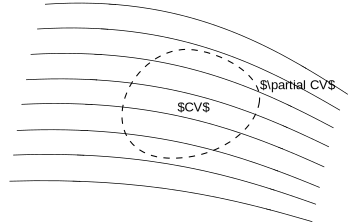
\includegraphics{fig/controlevolumes/Controlevolume_met_stroomlijnen}
  		\end{frame}
%%%%%%%%%%%%%%%%%%%%%%%%%%%%%%%%%%%%%%%%%%%%%%%%%%%%%%%%%%%%%%%%%%%%%%%%%%%
  		\begin{frame}
			\frametitle{Behoud van massa}
			\vspace{2cm}
			\begin{equation*}
				\left[
					\begin{array}{c}
						\mbox{De verandering} \\ \mbox{van massa in} \\ \mbox{het controlevolume}
					\end{array}
				\right]
				+
				\left[
					\begin{array}{c}
						\mbox{De netto} \\ \mbox{massastroom uit} \\ \mbox{het controlevolume}
					\end{array}
				\right]
				= 0
			\end{equation*}
		\end{frame}	
%%%%%%%%%%%%%%%%%%%%%%%%%%%%%%%%%%%%%%%%%%%%%%%%%%%%%%%%%%%%%%%%%%%%%%%%%%%
		\begin{frame}
			\frametitle{Massastroom}
			\vspace{1cm}
			\center
			\includegraphics{fig/controlevolumes/massastroom}
  		\end{frame}
%%%%%%%%%%%%%%%%%%%%%%%%%%%%%%%%%%%%%%%%%%%%%%%%%%%%%%%%%%%%%%%%%%%%%%%%%%%
  		\begin{frame}
  			\frametitle{Massastroom}
  			\begin{equation*}
				\Delta m = \rho \Delta x_{\perp} \diff A
			\end{equation*}
  			
  			\pause
  			\begin{equation*}
				\Delta m = \rho v_{\perp} \Delta t \diff A
			\end{equation*}
			
			\pause
  			\begin{equation*}
				\frac{\Delta m}{\Delta t} = \rho v_{\perp} \diff A
			\end{equation*}
			
			\pause
			\begin{equation}
				\diff \dot{m}  = \rho v_{\perp} \diff A
				\label{eqn:massastroom}
			\end{equation}
  		\end{frame}
%%%%%%%%%%%%%%%%%%%%%%%%%%%%%%%%%%%%%%%%%%%%%%%%%%%%%%%%%%%%%%%%%%%%%%%%%%%
		\begin{frame}
			\frametitle{Behoud van massa}
			\vspace{1cm}
			\begin{equation*}
				\left[
					\begin{array}{c}
						\mbox{De verandering} \\ \mbox{van massa in} \\ \mbox{het controlevolume}
					\end{array}
				\right]
				+
				\left[
					\begin{array}{c}
						\mbox{De netto} \\ \mbox{massastroom uit} \\ \mbox{het controlevolume}
					\end{array}
				\right]
				= 0
				\label{eqn:controlevolume,behoud van massa,woorden}
			\end{equation*}
			\vspace{1cm}
			\pause
			\begin{equation}
				\frac{\diff m_{CV}}{\diff t} + \dot{m}_{\partial CV} = 0
				\label{eqn:controlevolume,behoud van massa}
			\end{equation}
		\end{frame}	
%%%%%%%%%%%%%%%%%%%%%%%%%%%%%%%%%%%%%%%%%%%%%%%%%%%%%%%%%%%%%%%%%%%%%%%%%%%
  		\begin{frame}
			\frametitle{Behoud van impuls}
			\vspace{0.7cm}
			\begin{equation*}
				\left[
					\begin{array}{c}
						\mbox{De verandering} \\ \mbox{van impuls} \\ \mbox{in het}  \\ \mbox{controlevolume}
					\end{array}
				\right]
				+
				\left[
					\begin{array}{c}
						\mbox{De netto} \\ \mbox{impulsstroom} \\ \mbox{uit het} \\ \mbox{controlevolume}
					\end{array}
				\right]
				=
				\left[
					\begin{array}{c}
						\mbox{De totale} \\ \mbox{kracht} \\ \mbox{op het} \\ \mbox{controlevolume}
					\end{array}
				\right]
				\label{eqn:controlevolume,behoud van impuls,woorden}
			\end{equation*}
			\vspace{1cm}
			\pause
			\begin{equation}
				\frac{\diff \vt{P}_{CV}}{\diff t} + \dot{\vt{P}}_{\partial CV} =  \vt{F}
				\label{eqn:controlevolume,behoud van impuls}
			\end{equation}
		\end{frame}	
%%%%%%%%%%%%%%%%%%%%%%%%%%%%%%%%%%%%%%%%%%%%%%%%%%%%%%%%%%%%%%%%%%%%%%%%%%%
  		\begin{frame}
			\frametitle{Behoud van energie}
			\vspace{0.5cm}
			\begin{equation*}
				\left[
					\begin{array}{c}
						\mbox{De verandering} \\ \mbox{van energie} \\ \mbox{in het} \\ \mbox{controlevolume}
					\end{array}
				\right]
				+
				\left[
					\begin{array}{c}
						\mbox{De netto} \\ \mbox{energiestroom} \\ \mbox{uit het} \\ \mbox{controlevolume}
					\end{array}
				\right]
				=
				\left[
					\begin{array}{c}
						\mbox{De warmtesroom} \\ \mbox{toegevoegd en} \\   \mbox{arbeidsstroom} \\ \mbox{onttrokken aan } \\ \mbox{het controlevolume}
					\end{array}
				\right]
				\label{eqn:controlevolume,behoud van energie,woorden}
			\end{equation*}
			\vspace{1cm}
			\pause
			\begin{equation}
				\frac{\diff E_{CV}}{\diff t} + \dot{E}_{\partial CV} =  \dot{Q}-\dot{W}
				\label{eqn:controlevolume,behoud van energie}
			\end{equation}
		\end{frame}	
%%%%%%%%%%%%%%%%%%%%%%%%%%%%%%%%%%%%%%%%%%%%%%%%%%%%%%%%%%%%%%%%%%%%%%%%%%%
	\section{Controle volume met één instroming en één uitstroming}	
  		\begin{frame}
			\frametitle{Controle volume met één instroming en één uitstroming}
			\vspace{1cm}
			\centering
			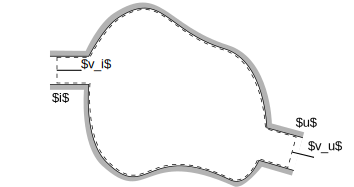
\includegraphics{fig/controlevolumes/Controlevolume_een_in_en_uitstroming}
		\end{frame}
%%%%%%%%%%%%%%%%%%%%%%%%%%%%%%%%%%%%%%%%%%%%%%%%%%%%%%%%%%%%%%%%%%%%%%%%%%%
  		\begin{frame}
			\frametitle{Controle volume met één instroming en één uitstroming}
			\begin{textblock}{5}(0,3)
            	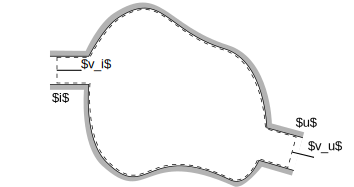
\includegraphics[width=5cm]{fig/controlevolumes/Controlevolume_een_in_en_uitstroming}
        	\end{textblock}
        	\vspace{2cm}
			\begin{equation}
				\rho_i v_{i,\perp} A_i = \rho_u v_{u,\perp} A_u
				\label{eqn:behoud van massa in een stationair controlevolume met een in en uitstroming}
			\end{equation}
			\pause
			\begin{align}
				F_{x,R} &= p_{u} A_u n_{x,u} - p_{i} A_i n_{x,i} + \dot{m} (v_{x,u}-v_{x,i}) \nonumber \\
				F_{y,R} &= p_{u} A_u n_{y,u} - p_{i} A_i n_{y,i} + \dot{m} (v_{y,u}-v_{y,i}) \\
				F_{z,R} &= p_{u} A_u n_{z,u} - p_{i} A_i n_{z,i} + \dot{m} (v_{z,u}-v_{z,i}) \nonumber
				\label{eqn:behoud van impuls in een stationair controlevolume met een in en uitstroming geprojecteerd2}
			\end{align}
			\pause
			\begin{equation}
				\dot{m} (u_u + \frac{p_u}{\rho_u} + \frac{1}{2}v^2_u + g z_u) - \dot{m} (u_i + \frac{p_i}{\rho_i}+ \frac{1}{2}v^2_i + g z_i) = \dot{Q}-\dot{W}_a
				\label{eqn:behoud van energie in een controlevolume met een in en uitstroming asvermogen}
			\end{equation}
		\end{frame}
%%%%%%%%%%%%%%%%%%%%%%%%%%%%%%%%%%%%%%%%%%%%%%%%%%%%%%%%%%%%%%%%%%%%%%%%%%%
		\begin{frame}
			\frametitle{Toepassing}
			\vspace{1cm}
			\centering
			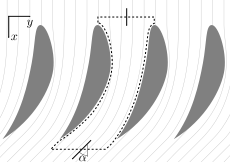
\includegraphics{fig/controlevolumes/Schoepenrij}
			
			Bepaal de horizontale en verticale kracht op één schoep, veronderstel isotherme stroming zonder warmteoverdracht
		\end{frame}
%%%%%%%%%%%%%%%%%%%%%%%%%%%%%%%%%%%%%%%%%%%%%%%%%%%%%%%%%%%%%%%%%%%%%%%%%%%
\end{document}